\section{Scope}
\begin{frame}{Scope}
\begin{itemize}
\item Antaget mulighed for overhaling af langsomtkørende biler

\item Kørsel uden for spidsbelastningerne
\item Individuel udbytte uafhændig af penetrationsraten
\item Minimal påvirkning af øvrig trafik
\end{itemize}
\end{frame}

\section{Fremtid}
\begin{frame}{Fremtid}


\begin{center}
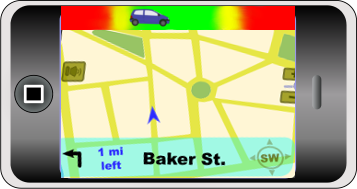
\includegraphics[width=1\textwidth]{images/product.png}
\end{center}
\end{frame}

\begin{frame}{Fremtid}
\begin{itemize}
\item 1. Simulering med præcise data
	\begin{itemize}
	\item Log af traffik lys
	\item Trængselsestimater (OD matrix)
	\end{itemize}
\item 2. Smartphone applikation
	\begin{itemize}
	\item Adgang til læsning af den aktuelle signalsætning
	\end{itemize}
\end{itemize}

\end{frame}

\begin{frame}{Konklusion}

\begin{itemize}
\item Op til 25\% besparelse af brænstof
\item Lille invistering
\item Individuel udbytte uafhændig af penetrationsraten
\item Minimal påvirkning af øvrig trafik
\end{itemize}
\end{frame}
